\documentclass[a4paper,12pt]{report}
\usepackage{color}
\usepackage{graphicx}
\usepackage{epstopdf}
\usepackage{amsmath}
\usepackage[table,xcdraw]{xcolor}
\usepackage{amssymb}
\usepackage{listings}
\definecolor{anti-flashwhite}{rgb}{0.95, 0.95, 0.96}
\lstset{ 
  backgroundcolor=\color{anti-flashwhite}
  }
\begin{document}
\title{
Operating Systems - 1: CS3510\\~\\
\begin{large}
Programming Assignment 2:\\Multi-Process \&
Multi-Threaded\\Computation of Statistics~\\
\end{large}
\begin{large}
Assignment Report
\end{large}
}
\author{Sagar Jain - CS17BTECH11034\\}
\maketitle
\section*{Program Design}
\subsection*{Using Processes}
The following points describe the code in detail.\\
\begin{enumerate}
\item The file Assgn2-ProcStat-CS17BTECH11034.cpp begins by including the
necessay libraries for input-output, few system calls(creating processes), algorithms and file systems.
\item First we create a struct to store in the shared memory, \textbf{\textit{stats}}.
\item In main, we start off by initilizing the following,
\begin{enumerate}
\item \textbf{\textit{SIZE}} i.e. the size of the shared memory we would like to create.
\item \textit{\textbf{name}} i.e. the name of the shared memory object to be created
or opened.
\item \textit{\textbf{fd}} i.e. a nonnegative value, the file descriptor of the shared memory object created.
\item \textit{\textbf{ptr}} i.e. a pointer to the mapped shared area.
\item \textit{\textbf{pid}} to store the pid when a process is forked.
\end{enumerate}
\item We then call shm open to create a new shared memory region. We
use the arguments O CREAT / O RDWR to create a new shared
memory object if one doesn’t already exist and open the object for
read-write access.On success, shm open returns a nonnegative file descriptor and we store it in fd.
\item We then check for errors in creating of the shared memory.
\item We then truncate the file to the required size in bytes, using ftruncate.
\item Then using mmap we store the value of the pointer to the mapped
shared area in ptr. We use the argument PROT READ / PROT WRITE
to allow both read and write access. We use MAP SHARED since
we want to share the mapping.
\item We type cast \textbf{\textit{ptr}} into \textbf{\textit{*stats}} and assign it to \textbf{\textit{statsistics}}.
\item We then use \textbf{\textit{cin}} to take input from user/file and store the numbers in a \textbf{\textit{vector}}.
\item Now we use fork() to create a new child process and using the value of pid we differentiate between the child and the parent process.In the child process we then compute the mean using a loop. We store the value of the computed mean into the shared memory using the pointer statisctics.
\item In the parent process we once again use fork() to create a new child process. In this chiild process we compute the standard deviation using two for loops. Once again we store the computed standard deviation into the shared memory using the pointer statistics.
\item In the parent process we use \textit{\textbf{fork}} once again to create another child process. In this child process we compute he median of the given numbers using the \textit{\textbf{sort}} function. Once we have the median of the data we store it into the shared memory using the pointer statistics.
\item At every \textit{\textbf{fork}} we use the value of the variable pid to differentiate between the child process and the parent process.
\item Now in the parent process we wait for the three child processes to terminate by invoking three \textit{\textbf{wait}} calls. 
\item Once the three child processes terminate we can start writing the output safely from the shared memory into the file.
\item We use \textit{\textbf{ofstream}} to write the output into the file.
\end{enumerate}
\subsection*{Using Threads}
\begin{enumerate}
\item The file Assgn2-ThStat-CS17BTECH11034.cpp begins by including the
necessay libraries for input-output, few system calls(creating threads), algorithms and file systems.
\item We first declare the following global varibales,
\begin{enumerate}
\item \textit{\textbf{mean}}
\item \textit{\textbf{median}}
\item \textit{\textbf{standard\_deviation}}
\end{enumerate}
\item Now we define the functions we need to compute the required statistics.
\item All the three functions return \textit{\textbf{void*}} and take only one parameter \textbf{\textit{void*}} as specified by the pthred signature.
\item In the functions we cast the void pointer into vector pointer and dereference this to perform any operations.
\item In all the three functions we end by calling \textit{\textbf{pthread\_exit}} this signifies the end of the thread.
\item In \textit{\textbf{main}}, we start off by initilizing the following,
\begin{enumerate}
\item \textit{\textbf{n}}, the number of numbers in the input.
\item \textit{\textbf{nums}}, a vector to store all the numbers.
\item \textbf{\textit{tid1}}, \textbf{\textit{tid2}}, \textbf{\textit{tid3}} the ids of the threads we would be creating.
\item We also initialize the default attributes using \textit{\textbf{pthread\_attr\_init}}.
\end{enumerate}
\item Now using \textbf{\textit{pthread\_create}} we create three threads to perform the tasks parallely.
\item  \textit{\textbf{pthread\_create}} takes in four arguments,
\begin{enumerate}
\item Pointer to a \textit{\textbf{pthread\_t variable}}, i.e. pointer to the variable storing tid.
\item Pointer to a \textit{\textbf{pthread\_attr\_t}} variable storing the attributes for the creation of the pthread.
\item Name of the function to be called by the thread, this function must be a \textbf{\textit{void*}} returing function, and it must accept only one argument of type \textit{\textbf{void*}}.
\item The \textit{\textbf{void*}} type argument to the fucntion.
\end{enumerate}
\item We then use \textit{\textbf{pthread\_join}} to wait for all the the pthreads to terminate.
\item Once all the pthreads have terminated, we can safely assume that all the global variables have been updated with the required values.
\item Now, we proceed to write the values into the file.
\item We write the output into the file using \textit{\textbf{ofstream}} and \textbf{\textit{cout}}.
\end{enumerate}
\subsubsection*{Note}
For both the programs, the commented out lines are used to measure the total time taken by the code, I have used \textit{\textbf{chrono}} to accomplish this task.
\newpage
\section*{Output Analysis}
The following is the output for both the programs,\\\\
\begin{tabular}{|c|c|c|c|}
\hline
Input Size & Test Cases       & Mean Time - Threads (us)          & Mean Time - Processes (us) \\ \hline
10         & \cellcolor[HTML]{FFFFFF}10 & \cellcolor[HTML]{FFFFFF}907  & 2282                  \\ \hline
100        & \cellcolor[HTML]{FFFFFF}10 & \cellcolor[HTML]{FFFFFF}1142 & 2376                  \\ \hline
1000       & 10                         & 4604                         & 5342                  \\ \hline
10000      & 10                         & 47103                        & 39059                 \\ \hline
100000     & 10                         & 204933                       & 183488                \\ \hline
200000     & 10                         & 219885                       & 186505                \\ \hline
300000     & 10                         & 417203                       & 373982                \\ \hline
400000     & 10                         & 583214                       & 457077                \\ \hline
500000     & 10                         & 761222                       & 622016                \\ \hline
600000     & 10                         & 781995                       & 678334                \\ \hline
\end{tabular}
\begin{center}
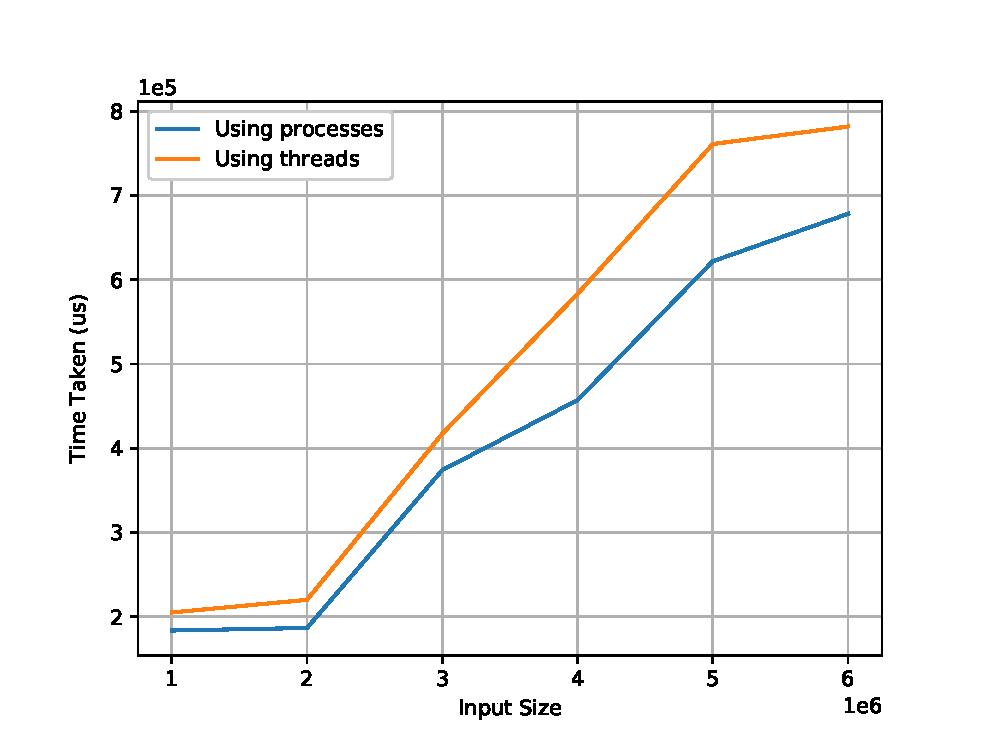
\includegraphics{process_vs_thread.eps}
\end{center}
The above is the plot of the execution times for both programs.
\newpage
\begin{enumerate}  
\item The given plot shows the execution time of the two programs for different inout sizes. The output times are in microseconds.
\item It is evident that the total time taken increases with increase in input size for both the programs.
\item It is clear to see that the program using processes to compute the statistics performs better at large inputs.
\item Not only does the program using processes perform better but the difference in the performance widens with increase in input size.
\item For inputs of the order of $10^6$, the program using processes executes around $25\%$ faster than the one using threads.
\item The following is the plot of time takens by both the programs to execute for smaller inputs.
\end{enumerate}
\begin{center}
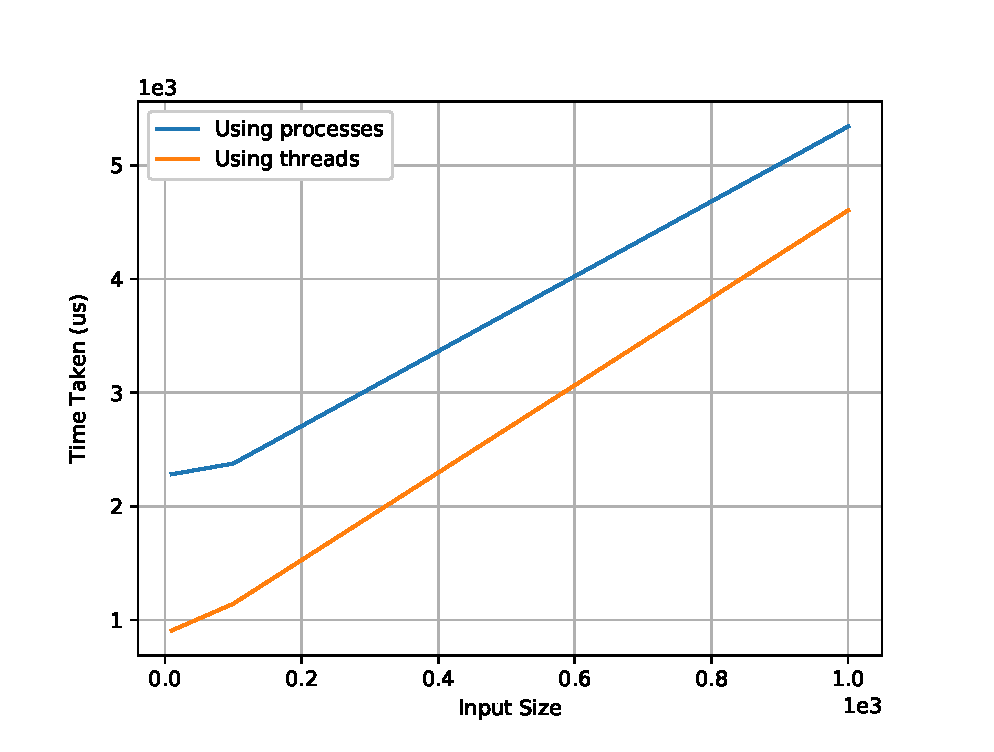
\includegraphics{thread_early_domination.eps}
\end{center}
\newpage
\subsection*{Explaination of Results}
\begin{enumerate}
\item Before commenting on the different times taken, it must be noted that in linux, a process is not too different from a thread. The system call\textit{ \textbf{clone}} clones a task, with a configurable level of sharing, it is only in this level of sharing that a process and thread are different.
\item Performance of threads and processes may be different in other operating systems, depending on the way the two are implemented.
\item At a small input size, we see that threads perform better, this could be due to the following reasons,
\begin{enumerate}
\item Faster Context Switch between threads.
\item Since threads have the same address space, writing to the same address space is faster than writing to a shared memory space as is the case with IPC.
\end{enumerate}
\item As we move to larger input sizes, the execution time of the program using processes gets better than the one using threads, this can be due to the fact that a process essentially has more resources than a thread($\because$ less sharing of resouces), therefore for heavy computation it performs better than a thread.
\item From the gathered results, a thread could be considered as \textit{lite} process.
\end{enumerate}
\end{document}